\documentclass{article}
\usepackage{titling}
\usepackage{lipsum}
\usepackage{amsmath}
\usepackage{listings}
\usepackage{graphicx}
\usepackage{subcaption}
\usepackage{pgfplots}
\usepackage[margin=1in]{geometry}
\usepgfplotslibrary{statistics}



\begin{document}
\noindent
\begin{minipage}[t]{0.6\textwidth}
    \begin{flushleft}
        \LARGE\textbf{Math 343 - Homework 4} \\
        \vspace{6pt} % add 6pt of vertical space
        \hrule width 10cm
        \vspace{12pt}
        \large\textbf{Preston Duffield} \\
        \large Western Washington University \\
        \today
        % April 18, 2023
        \vspace{24pt}
    \end{flushleft}
\end{minipage}

\section*{Question 1}

\subsection*{a)}

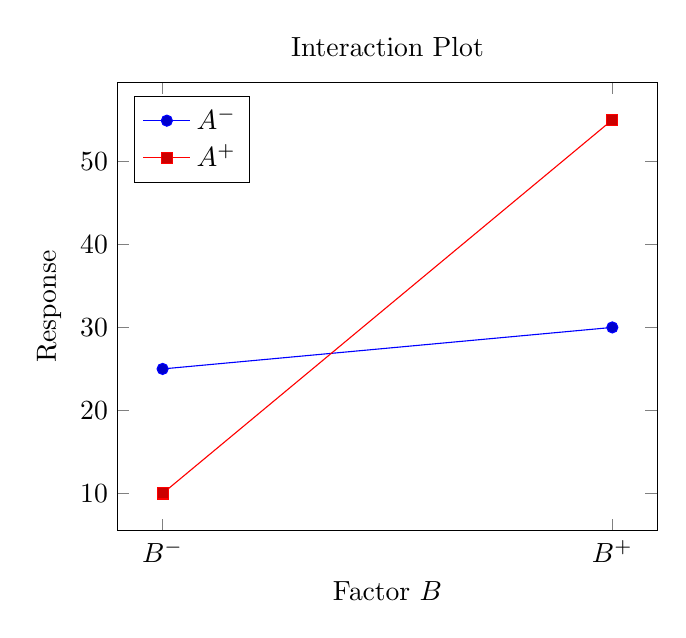
\begin{tikzpicture}
    \begin{axis}[
        title={Interaction Plot},
        xlabel={Factor $B$},
        ylabel={Response},
        symbolic x coords={$B^{-}$, $B^{+}$},
        xtick=data,
        legend pos=north west
    ]
    \addplot coordinates {($B^{-}$, 25) ($B^{+}$, 30)};
    \addplot coordinates {($B^{-}$, 10) ($B^{+}$, 55)};
    \legend{$A^{-}$,$A^{+}$}
    \end{axis}
\end{tikzpicture}

Since the Lines in the interaction plot are not parallel, this indicates interaction.


\subsection*{b)}
\begin{flushleft}
The Main Effect of $A$ is:
\end{flushleft}
\begin{align*}
    A & = \bar{y}_{A^{+}} - \bar{y}_{A^{-}} \\
      & = \frac{\mu_{22} + \mu_{21}}{2} - \frac{\mu_{12} + \mu_{11}}{2} \\
      & = \frac{55 + 10}{2} - \frac{30 + 25}{2} \\
      & = 5
\end{align*}
\begin{flushleft}
The Main Effect of $B$ is:
\end{flushleft}
\begin{align*}
    B & = \bar{y}_{B^{+}} - \bar{y}_{B^{-}} \\
      & = \frac{\mu_{12} + \mu_{22}}{2} - \frac{\mu_{11} + \mu_{21}}{2} \\
      & = \frac{30 + 55}{2} - \frac{25 + 10}{2} \\
      & = 25
\end{align*}
\begin{flushleft}
The Interaction Effect of $A$ and $B$ is:
\end{flushleft}
\begin{align*}
    AB & = \frac{\mu_{22} + \mu_{11}}{2} - \frac{\mu_{21} + \mu_{12}}{2} \\
       & = \frac{55 + 25}{2} - \frac{10 + 30}{2} \\
       & = 20
\end{align*}

\section*{Question 2}

\subsection*{a)}
\textbf{Two-way ANOVA: y versus, A, B} \\
Note that calculated values are bold.
\begin{equation*}
\begin{array}{c|c|c|c|c|c}
    \text{Source} &\text{DF}& \text{SS} & \text{MS} & \text{F} &\text{P}  \\
    \hline
    \text{A} & \text{1} & \text{0.322} & \textbf{-} & \textbf{-} &\textbf{-}  \\
    \text{B} & \textbf{-} & \text{80.554} & \text{40.2771} & \text{4.59} &\textbf{-}  \\
    \text{Interaction} & \textbf{-}  & \textbf{-} & \textbf{-} & \textbf{-} &\textbf{-}  \\
    \text{Error} & \text{12} & \text{105.327} & \text{8.7773} & \textbf{-} &\textbf{-}  \\
    \text{Total} & \text{17}  & \text{231.551} &  &  &  \\

\end{array}
\end{equation*}\\

\subsection*{b)}
\subsection*{c)}
\subsection*{d)}

\section*{Question 3}

\subsection*{b)}

% \begin{figure}[h]
%     \centering
%     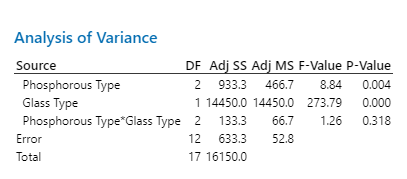
\includegraphics[width=0.5\textwidth]{./images/3_b.png}
%     \caption{Anova table from Minitab.}
%     \label{fig:3_B}
% \end{figure}
% \begin{figure}[h]
%     \centering
%     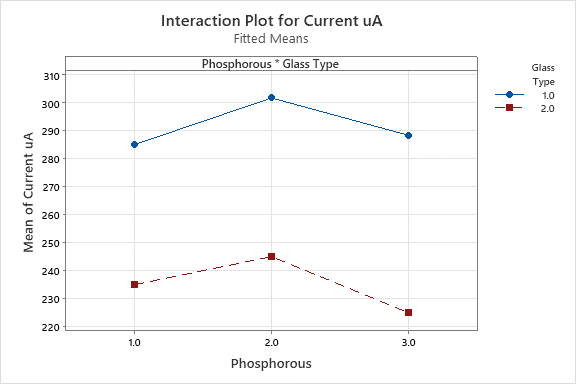
\includegraphics[width=0.5\textwidth]{./images/3_b_2.png}
%     \caption{Anova table from Minitab.}
%     \label{fig:3_b_2}
% \end{figure}

\begin{figure}[h]
    \centering
    \begin{subfigure}[b]{0.4\textwidth}
        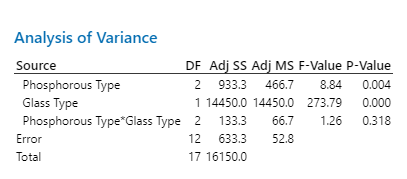
\includegraphics[width=1\textwidth]{./images/3_b.png}
        \caption{Anova table from Minitab.}
      \label{fig:img1}
    \end{subfigure}
    \hfill
    \begin{subfigure}[b]{0.5\textwidth}
        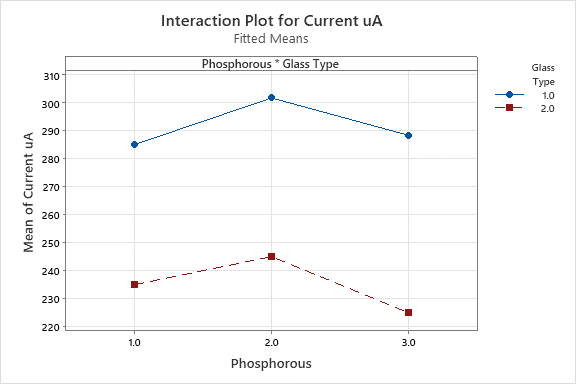
\includegraphics[width=1\textwidth]{./images/3_b_2.png}
        \caption{Interaction plot from Minitab.}
      \label{fig:img2}
    \end{subfigure}
    \label{fig:both}
\end{figure}

\begin{flushleft}
    $H_0$: $(\tau \beta)_{11} = (\tau \beta)_{12} = (\tau \beta)_{22} = (\tau \beta)_{21} = 0$ \\
    $H_a$: At least one $(\tau \beta)_{ij}$ is different.\\
\end{flushleft}

Since the p-value for the interaction of the two factors is $0.318 > \alpha = 0.05$, we can conclude the following.
There is not enough evidence to support the hypotheis that at least one $(\tau \beta)_{ij}$ is different,
ie, there does not exist interaction between the two factors. 

\clearpage
\subsection*{c)}
\begin{figure}[h]
    \centering
    \begin{subfigure}[b]{0.45\textwidth}
        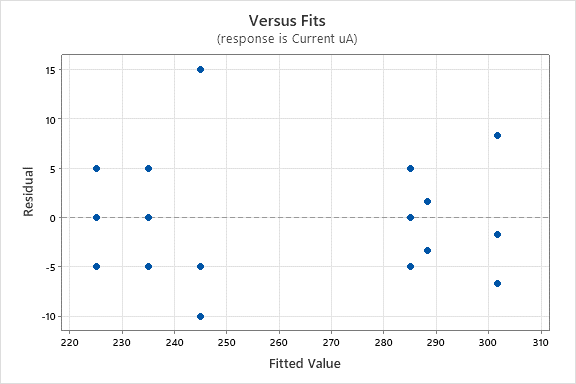
\includegraphics[width=1\textwidth]{./images/3_c_1.png}
        \caption{Residuals versus fits plot from Minitab.}
      \label{fig:img11}
    \end{subfigure}
    \hfill
    \begin{subfigure}[b]{0.45\textwidth}
        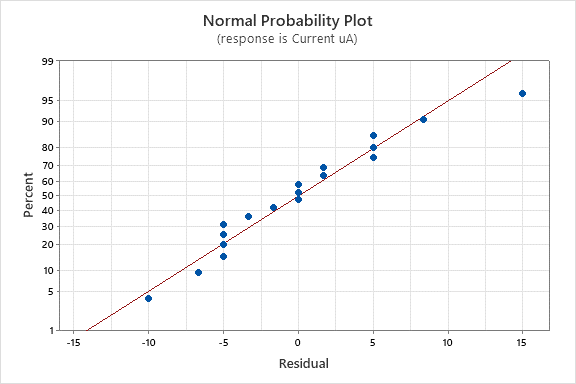
\includegraphics[width=1\textwidth]{./images/3_c_2.png}
        \caption{Normal probability plot from Minitab.}
      \label{fig:img22}
    \end{subfigure}
    \label{fig:both}
\end{figure}
The residual plot does not seem to indicate heteroskedasticity. The normal probability plot appears to follow a stright line, indicating normality.
These two plots indicate that the model assumptions are satified.
\subsection*{d)}
\begin{flushleft}
    $H_0$: $\tau_1 = \tau_2 = \tau_3 = 0$ \\
    $H_a$: At least one $\tau_i$ is different.\\
\end{flushleft}
Since the p-value is $0.004 < \alpha = 0.05$, we can conclude the following. \\
There is enough statistic evidence to support at least one $\tau_i$ being different.
% This is significant so do a tukeys pairwise.
\\
\textbf{a Tukey’s test for pairwise comparison} \\
\begin{equation*}
    \begin{array}{c|c|c}
        \text{Phosphorous Type} &\text{N}& \text{Mean} \\
        \hline
        1 & 6 & \frac{285+235}{2} = 260\\
        2 & 6 & \frac{301.67+245}{2} = 273.335\\
        3 & 6 & \frac{288.33+225}{2} = 256.665\\
    
    \end{array}
    \end{equation*}\\
\begin{flushleft}
    The difference in means are:
\end{flushleft}
\begin{equation*}
    \begin{array}{c|c}
        \text{Difference of Types} &\text{Difference}\\
        \hline
        2 - 1 & 273.335 - 260 = 13.335\\
        3 - 1 & 256.665 - 260 = -3.335\\
        3 - 2 & 256.665 - 273.335 = -16.67\\
    
    \end{array}
    \end{equation*}\\

\subsection*{e)}

\section*{Question 4}

\section*{Question 5}

\section*{Question 6}

\section*{Question 7}



\end{document}
